% Created by tikzDevice version 0.10.1 on 2016-07-26 20:48:00
% !TEX encoding = UTF-8 Unicode
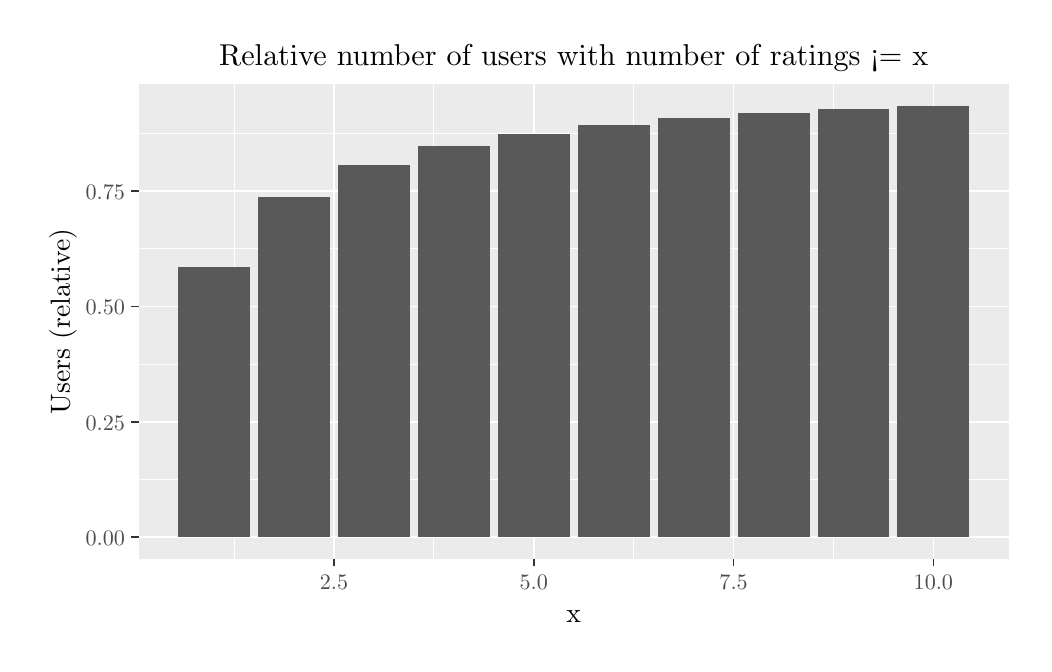
\begin{tikzpicture}[x=1pt,y=1pt]
\definecolor{fillColor}{RGB}{255,255,255}
\path[use as bounding box,fill=fillColor,fill opacity=0.00] (0,0) rectangle (360.07,222.54);
\begin{scope}
\path[clip] (  0.00,  0.00) rectangle (360.07,222.54);
\definecolor{drawColor}{RGB}{255,255,255}
\definecolor{fillColor}{RGB}{255,255,255}

\path[draw=drawColor,line width= 0.6pt,line join=round,line cap=round,fill=fillColor] (  0.00,  0.00) rectangle (360.07,222.54);
\end{scope}
\begin{scope}
\path[clip] ( 40.08, 30.62) rectangle (354.57,202.21);
\definecolor{fillColor}{gray}{0.92}

\path[fill=fillColor] ( 40.08, 30.62) rectangle (354.57,202.21);
\definecolor{drawColor}{RGB}{255,255,255}

\path[draw=drawColor,line width= 0.3pt,line join=round] ( 40.08, 59.27) --
	(354.57, 59.27);

\path[draw=drawColor,line width= 0.3pt,line join=round] ( 40.08,100.95) --
	(354.57,100.95);

\path[draw=drawColor,line width= 0.3pt,line join=round] ( 40.08,142.64) --
	(354.57,142.64);

\path[draw=drawColor,line width= 0.3pt,line join=round] ( 40.08,184.33) --
	(354.57,184.33);

\path[draw=drawColor,line width= 0.3pt,line join=round] ( 74.59, 30.62) --
	( 74.59,202.21);

\path[draw=drawColor,line width= 0.3pt,line join=round] (146.79, 30.62) --
	(146.79,202.21);

\path[draw=drawColor,line width= 0.3pt,line join=round] (218.98, 30.62) --
	(218.98,202.21);

\path[draw=drawColor,line width= 0.3pt,line join=round] (291.18, 30.62) --
	(291.18,202.21);

\path[draw=drawColor,line width= 0.6pt,line join=round] ( 40.08, 38.42) --
	(354.57, 38.42);

\path[draw=drawColor,line width= 0.6pt,line join=round] ( 40.08, 80.11) --
	(354.57, 80.11);

\path[draw=drawColor,line width= 0.6pt,line join=round] ( 40.08,121.80) --
	(354.57,121.80);

\path[draw=drawColor,line width= 0.6pt,line join=round] ( 40.08,163.48) --
	(354.57,163.48);

\path[draw=drawColor,line width= 0.6pt,line join=round] (110.69, 30.62) --
	(110.69,202.21);

\path[draw=drawColor,line width= 0.6pt,line join=round] (182.88, 30.62) --
	(182.88,202.21);

\path[draw=drawColor,line width= 0.6pt,line join=round] (255.08, 30.62) --
	(255.08,202.21);

\path[draw=drawColor,line width= 0.6pt,line join=round] (327.28, 30.62) --
	(327.28,202.21);
\definecolor{fillColor}{gray}{0.35}

\path[fill=fillColor] ( 54.37, 38.42) rectangle ( 80.36,136.20);

\path[fill=fillColor] ( 83.25, 38.42) rectangle (109.24,161.22);

\path[fill=fillColor] (112.13, 38.42) rectangle (138.12,172.82);

\path[fill=fillColor] (141.01, 38.42) rectangle (167.00,179.68);

\path[fill=fillColor] (169.89, 38.42) rectangle (195.88,184.16);

\path[fill=fillColor] (198.77, 38.42) rectangle (224.76,187.38);

\path[fill=fillColor] (227.65, 38.42) rectangle (253.64,189.82);

\path[fill=fillColor] (256.53, 38.42) rectangle (282.52,191.71);

\path[fill=fillColor] (285.41, 38.42) rectangle (311.40,193.18);

\path[fill=fillColor] (314.28, 38.42) rectangle (340.28,194.41);
\end{scope}
\begin{scope}
\path[clip] (  0.00,  0.00) rectangle (360.07,222.54);
\definecolor{drawColor}{gray}{0.30}

\node[text=drawColor,anchor=base east,inner sep=0pt, outer sep=0pt, scale=  0.80] at ( 35.13, 35.41) {0.00};

\node[text=drawColor,anchor=base east,inner sep=0pt, outer sep=0pt, scale=  0.80] at ( 35.13, 77.09) {0.25};

\node[text=drawColor,anchor=base east,inner sep=0pt, outer sep=0pt, scale=  0.80] at ( 35.13,118.78) {0.50};

\node[text=drawColor,anchor=base east,inner sep=0pt, outer sep=0pt, scale=  0.80] at ( 35.13,160.47) {0.75};
\end{scope}
\begin{scope}
\path[clip] (  0.00,  0.00) rectangle (360.07,222.54);
\definecolor{drawColor}{gray}{0.20}

\path[draw=drawColor,line width= 0.6pt,line join=round] ( 37.33, 38.42) --
	( 40.08, 38.42);

\path[draw=drawColor,line width= 0.6pt,line join=round] ( 37.33, 80.11) --
	( 40.08, 80.11);

\path[draw=drawColor,line width= 0.6pt,line join=round] ( 37.33,121.80) --
	( 40.08,121.80);

\path[draw=drawColor,line width= 0.6pt,line join=round] ( 37.33,163.48) --
	( 40.08,163.48);
\end{scope}
\begin{scope}
\path[clip] (  0.00,  0.00) rectangle (360.07,222.54);
\definecolor{drawColor}{gray}{0.20}

\path[draw=drawColor,line width= 0.6pt,line join=round] (110.69, 27.87) --
	(110.69, 30.62);

\path[draw=drawColor,line width= 0.6pt,line join=round] (182.88, 27.87) --
	(182.88, 30.62);

\path[draw=drawColor,line width= 0.6pt,line join=round] (255.08, 27.87) --
	(255.08, 30.62);

\path[draw=drawColor,line width= 0.6pt,line join=round] (327.28, 27.87) --
	(327.28, 30.62);
\end{scope}
\begin{scope}
\path[clip] (  0.00,  0.00) rectangle (360.07,222.54);
\definecolor{drawColor}{gray}{0.30}

\node[text=drawColor,anchor=base,inner sep=0pt, outer sep=0pt, scale=  0.80] at (110.69, 19.64) {2.5};

\node[text=drawColor,anchor=base,inner sep=0pt, outer sep=0pt, scale=  0.80] at (182.88, 19.64) {5.0};

\node[text=drawColor,anchor=base,inner sep=0pt, outer sep=0pt, scale=  0.80] at (255.08, 19.64) {7.5};

\node[text=drawColor,anchor=base,inner sep=0pt, outer sep=0pt, scale=  0.80] at (327.28, 19.64) {10.0};
\end{scope}
\begin{scope}
\path[clip] (  0.00,  0.00) rectangle (360.07,222.54);
\definecolor{drawColor}{RGB}{0,0,0}

\node[text=drawColor,anchor=base,inner sep=0pt, outer sep=0pt, scale=  1.00] at (197.32,  7.70) {x};
\end{scope}
\begin{scope}
\path[clip] (  0.00,  0.00) rectangle (360.07,222.54);
\definecolor{drawColor}{RGB}{0,0,0}

\node[text=drawColor,rotate= 90.00,anchor=base,inner sep=0pt, outer sep=0pt, scale=  1.00] at ( 15.24,116.42) {Users (relative)};
\end{scope}
\begin{scope}
\path[clip] (  0.00,  0.00) rectangle (360.07,222.54);
\definecolor{drawColor}{RGB}{0,0,0}

\node[text=drawColor,anchor=base,inner sep=0pt, outer sep=0pt, scale=  1.09] at (197.32,208.81) {Relative number of users with number of ratings <= x};
\end{scope}
\end{tikzpicture}
